\section{Gestionare Drafturi}\label{spec:drafts}

La nivelul modelului, aceste opțiuni sunt reprezentate prin interfața \texttt{DraftsUseCase}. Atât funcționalitatea de listare, cât și cea de editare se folosesc de funcționalitatea \emph{Room} prin care atunci când apare o modificare la nivelul bazei de date, o nouă valoare este emisă pentru interogările deja executate. Astfel, este ușoară o implementare reactivă pentru aceste funcționalități.

\lstinputlisting[style=javaCodeStyle, caption=Interfața Drafts Use Case]{./code/DraftsUseCase.kt}

Editarea câmpurilor text se face în manieră \emph{on the fly}, ceea ce înseamnă că nu este necesar un ecran separat drept formular și apăsarea unui buton de persistare a modificărilor. Aceasta se realizează înregistrând un \emph{callback} pe câmpurile de text, care apelează funcția de update. Această abordare ridică problema unor fluxuri de date mult prea rapide. De aceea, asupra fluxului de modificări este aplicat operatorul RxJava \texttt{throttleLast}. Figura \ref{fig:throttle}, din documentația RxJava \cite{ThrottleLast} ilustrează modul în care acest operator funcționează.

\begin{figure}[h]
  \centering
  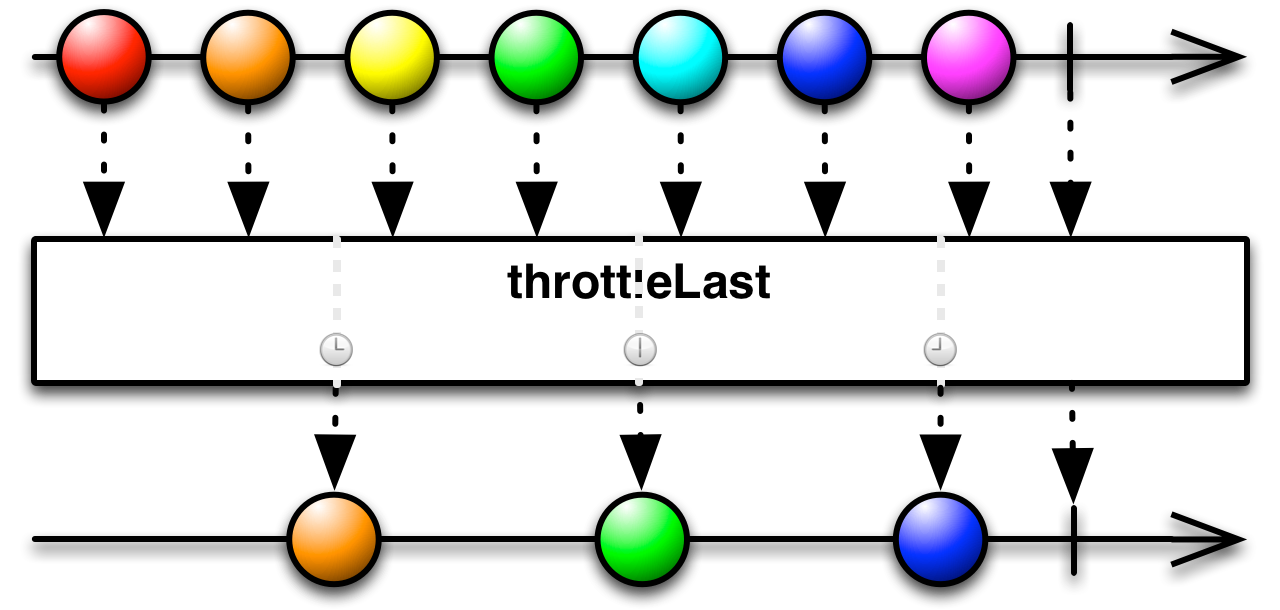
\includegraphics[width=0.7\textwidth]{throttleLast.png}
  \caption{Ilustrație throttleLast}
  \label{fig:throttle}
\end{figure}

În continuare este prezentată utilizarea operatorului \texttt{throttleLast}, împreună cu un exemplu de utilizare. Funcția \texttt{throttled} primește argumentele pentru aplicarea operatorului și o funcție și returnează o nouă funcție care are aceeași signatură, același comportament, dar executată la o rată de timp specificată. În acest mod sunt exemplificate funcțiile de ordin înalt și abilitatea de a reprezenta funcțiile ca valori în limbajul Kotlin.

\lstinputlisting[style=javaCodeStyle, caption=Funcții throttled]{./code/ThrottleImplementation.kt}
